\section{Problème de Cauchy pour l'équation biharmonique}\label{sec:problème-de-cauchy-pour-l'équation-biharmonique}

Soit $\Omega\subset\mathds{R}^2$ de frontière $\Gamma = \Gamma_0 \cup \Gamma_1$ tel que $\Gamma_0,\Gamma_1 \neq
\emptyset$ et $\Gamma_0 \bigcap \Gamma_1 = \emptyset$.
On étudie alors le problème suivant:
\begin{align}
	\label{CauchyPB}
	\left\{
	\begin{array}{r c l}
		\Delta^2u &= 0 ~\text{ dans }~ \Omega\\
		u&=u_0 ~\text{ sur }~ \Gamma_0\\
		\frac{\partial u}{\partial n} &= u^\prime_0 ~\text{ sur }~ \Gamma_0 \\
		\Delta u &= \omega_0 ~\text{ sur }~ \Gamma_0\\
		\frac{\partial\Delta u}{\partial n}&=\omega^\prime_0 ~\text{ sur }~ \Gamma_0
	\end{array}
	\right.
\end{align}
On cherche alors à résoudre le problème de Cauchy\ref{CauchyPB} .
Pour ce faire, on veut déterminer l'intégralité des conditions sur le bord, puis trouver la solution à l'intérieur du
domaine.

Pour des conditions correctes sur le bord, le problème\ref{CauchyPB} admet une unique solution.

On commence par décomposer le problème.
Pour ce faire, on pose $ \Delta u = \omega$ .
On obtient alors le problème suivant:
\begin{align}
	\label{CauchyPB2}
	\left\{
	\begin{array}{r c l}
		\Delta u &= \omega  ~\text{ dans }~ \Omega\\
		\Delta\omega&=0 ~\text{ sur }~ \Omega\\
		u&=u_0 ~\text{ sur }~ \Gamma_0\\
		\frac{\partial u}{\partial n} &= u^\prime_0 ~\text{ sur }~ \Gamma_0 \\
		\Delta u &= \omega_0 ~\text{ sur }~ \Gamma_0\\
		\frac{\partial\Delta u}{\partial n}&=\omega^\prime_0 ~\text{ sur }~ \Gamma_0
	\end{array}
	\right.
\end{align}

On peut alors séparer le problème\ref{CauchyPB2} en deux problèmes inverse de Cauchy.

\begin{equation}
	\begin{array}{r c l}
		\left\{\begin{array}{r c l}
			       \Delta \omega &= 0 \text{ dans } \Omega \\
			       \omega &=\omega_0 \text{ sur } \Gamma_0\\
			       \frac{\partial \omega}{\partial n} &= \omega^\prime_0 \text{ sur } \Gamma_0
		\end{array}\right.

		& \text{ et } &
		\left\{\begin{array}{r c l}
			       \Delta u &=  \omega \text{ dans } \Omega \\
			       u &=u_0 \text{ sur } \Gamma_0\\
			       \frac{\partial u}{\partial n} &= u^\prime_0 \text{ sur } \Gamma_0
		\end{array}\right.
	\end{array}
\end{equation}

\section{Résolution du problème}\label{sec:résolution-du-problème}
\subsection{Méthode 1}\label{subsec:méthode-1}
Pour résoudre le problème présenté, on s'interesse dans un premier temps à la méthode présentée par C. Tajani et H.
Kajtih et A. Daanoun.

Pour ce faire on implémente avec FreeFem l'algorithme décrit dans le papier donné en annexe.
On résout alors chaque problème à l'aide des éléments finis.
L'écriture sous forme variationnelle permet alors d'exprimer le problème sous une forme utilisable par FreeFem.

\subsubsection*{Algorithme 1}
Step 1: Specify an initial guess $\omega_{1}$ and $u_{1}$ on $\Gamma_{1}$.
Step 2: Solve the following mixed well-posed boundary value problems:
\begin{align*}
	\left\{\begin{array}{ll}
		       \Delta \omega^{(0)}=0 & \text { in } \Omega \\
		       \omega^{(0)}=\omega_{1} & \text { on } \Gamma_{1} \quad \text { and } \\
		       \frac{\partial \omega^{(0)}}{\partial n}=\omega_{0}^{\prime} & \text { on } \Gamma_{0}
	\end{array} \quad\left\{\begin{array}{ll}
		                        \Delta u^{(0)}=\omega^{(0)} & \text { in } \Omega \\
		                        u^{(0)}=u_{1} & \text { on } \Gamma_{1} \\
		                        \frac{\partial u^{(0)}}{\partial n}=u_{0}^{\prime} & \text { on } \Gamma_{0}
	\end{array}\right.\right.
\end{align*}


to obtain $\frac{\partial \omega^{(0)}}{\partial n}_{| \Gamma_{1}}=v_{1}$


to obtain $\frac{\partial u^{(0)}}{\partial n_{| \Gamma_{1}}}=h_{1}$


Step 3:
i) If the approximation $\left(u^{(2 k)}, \omega^{(2 k)}\right)$ is constructed, solve the two mixed wellposed boundary value problems:


$\left\{\begin{array}{ll}\Delta \omega^{(2 k+1)}=0 & \text { in } \Omega \\ \omega^{(2 k+1)}=\omega_{0} & \text { on } \Gamma_{0} \quad \text { and } \\ \frac{\partial \omega^{(2 k+1)}}{\partial n}=v_{k+1} & \text { on } \Gamma_{1}\end{array} \quad\left\{\begin{array}{ll}\Delta u^{(2 k+1)}=\omega^{(2 k+1)} & \text { in } \Omega \\ u^{(2 k+1)}=u_{0} & \text { on } \Gamma_{0} \\ \frac{\partial u^{(2 k+1)}}{\partial n} & =h_{k+1}\end{array} \quad \text { on } \Gamma_{1}\right.\right.$


to obtain $\quad \omega_{| \Gamma_{1}}^{(2 k+1)}=\omega_{k+2}$


to obtain $u_{| \Gamma_{1}}^{(2 k+1)}=u_{k+2}$


ii) If the approximation $\left(u^{(2 k+1)}, \omega^{(2 k+1)}\right)$ is constructed, solve alternatively
the two mixed well-posed boundary value problems:


$\left\{\begin{array}{ll}\Delta \omega^{(2 k+2)}=0 & \text { in } \Omega \\ \omega^{(2 k+2)}=\omega_{k+2} & \text { on } \Gamma_{1} \quad \text { and } \\ \frac{\partial \omega^{(2 k+2)}}{\partial n}^{(2+2)}=\omega_{0}^{\prime} & \text { on } \Gamma_{0}\end{array} \quad\left\{\begin{array}{ll}\triangle u^{(2 k+2)}=\omega^{(2 k+2)} & \text { in } \Omega \\ u^{(2 k+2)}=u_{k+2} & \text { on } \Gamma_{1} \\ \frac{\partial u}{\partial n}^{(2 k+2)}=u_{0}^{\prime} & \text { on } \Gamma_{0}\end{array}\right.\right.$


to obtain $\frac{\partial \omega^{(2 k+2)}}{\partial n | \Gamma_{1}}=v_{k+2}$


to obtain $\frac{\partial u^{(2 k+2)}}{\partial n | \Gamma_{1}}=h_{k+2}$


Step 4: Repeat step 3 for $k \geq 0$ until a specified stopping criterion is satisfied.



On peut facilement modifier l'appartenance des bords à la sous frontière $\Gamma_0$ ou  $\Gamma_1$, en utilisant le
label $1$ ou $2$ dans la définition des bords.


\subsection{Méthode 2}\label{subsec:méthode-2}
On s'intéresse à l'algorithme de Dirichlet-Neumann pénalisé barycentriquement.
Pour ce faire, on repart de la séparation du problème en deux problèmes, laplacien et poisson.
On peut alors résoudre une étape pour $\omega$, puis pour $u$.

On peut adapter cet algorithme en reprenant l'idée du premier.
C'est-à-dire que l'on résout les 2 problèmes itérativement de manière croisée.
Pour ce faire, on remplace l'étape dans la boucle pour la résolution de chauqe problème par celle proposé par
l'article introduisant la méthode.

Par contre, l'utilisation d'une méthode de Schwartz semble restreindre la forme du domaine et impose que pour une
forme rectangulaire, on a seulement un bord sans condition d'imposé.
Alors que pour la première méthode, il n'y a pas cette restriction.


\section{Verification résultat numérique}\label{sec:verification-résultat-numérique}

On commence par s'intéresser à la solution du problème homogène.
On obtient alors :

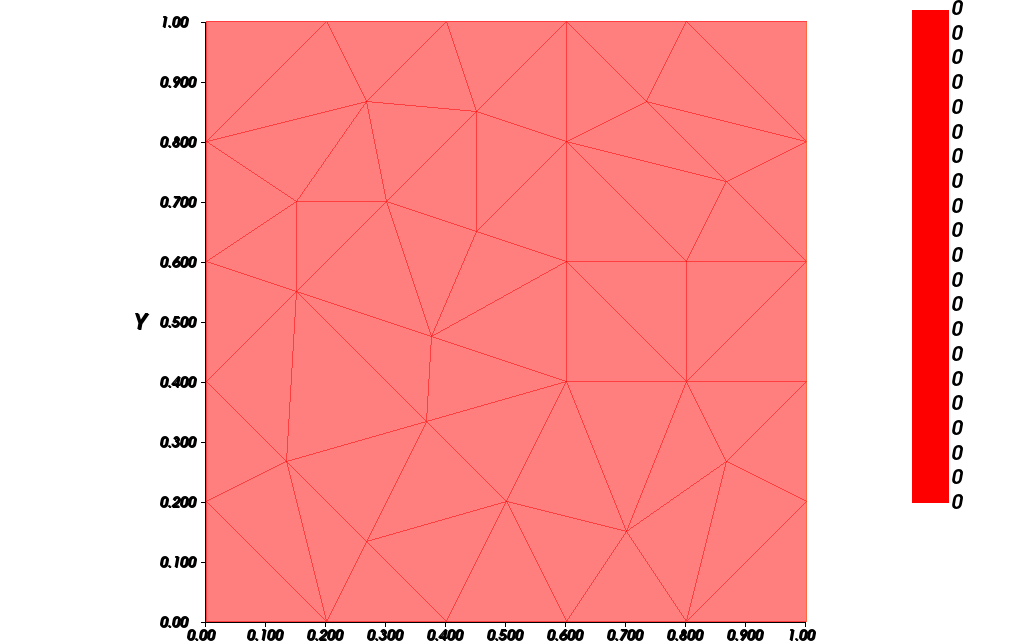
\includegraphics[scale=.5]{src/zero.png}

\section{Conclusion}\label{sec:conclusion}
L'implémentation de l'algorithme 1 se fait assez bien en FreeFem.
Il me semble qu'il ya quelques soucis au niveau des conditions de types Neumann sur la prise en compte de la dérivée.
